\documentclass{article}

\usepackage[margin=1in]{geometry}
\usepackage{amsmath,amsthm,amssymb}
\usepackage[spanish]{babel}
\usepackage{enumitem}
\usepackage{graphicx}
\usepackage{tikz}

\theoremstyle{plain}
\newtheorem{proposicion}{Proposición}[section]

\theoremstyle{definition}
\newtheorem{definition}{Definición}[section]

% Number sets
\newcommand{\R}{\mathbb{R}}
\newcommand{\Z}{\mathbb{Z}}
\newcommand{\N}{\mathbb{N}}
\newcommand{\Q}{\mathbb{Q}}
\newcommand{\C}{\mathbb{C}}

% Exercise environment
\newenvironment{ejercicio}[1]{\begin{trivlist}
\item[\hskip \labelsep {\bfseries Ejercicio}\hskip \labelsep {\bfseries #1.}]}{\end{trivlist}}

\setlist[enumerate,1]{label=(\alph*), leftmargin=*, itemsep=2pt}

\begin{document}

\title{Teoría de Grafos}
\author{Bustos Jordi\\Práctica I}

\maketitle

\begin{ejercicio}{1}
    Probar que, si \( G \) es un grafo simple, el número de aristas de \( G \) es menor o igual que \( n(n-1)/2 \), siendo \( n \) el número de vértices.
\end{ejercicio}
\begin{proof}

\end{proof}

\vspace{0.5cm}

\begin{ejercicio}{2}
    Dado \( n \) entero mayor o igual que 1, hallar una fórmula para la cantidad de grafos simples con conjunto de vértices \( \{1,\dots, n\} \). ¿En cuántos de esos grafos simples el grado del vértice 1 es menor o igual que 2? (la respuesta debe ser una expresión en función de \( n \) y completamente simplificada)
\end{ejercicio}
\begin{proof}

\end{proof}

\vspace{0.5cm}

\begin{ejercicio}{3}
    Un grafo \( G \) se dice conexo si, para todo par de vértices \( u \) y \( v \) de \( G \), existe una sucesión de vértices que comienza en \( u \), termina en \( v \) y tal que vértices consecutivos son adyacentes. Caso contrario, diremos que \( G \) es disconexo. Analizar si es verdadero o falso: el complemento de un grafo simple disconexo es conexo.
\end{ejercicio}
\begin{proof}

\end{proof}

\vspace{0.5cm}

\begin{ejercicio}{4}
    Determinar el tamaño máximo de un clique y el tamaño máximo de un conjunto independiente para el grafo de abajo. Justificar por qué no puede haber un clique o un conjunto independiente de tamaño mayor.
    \begin{center}
        \begin{tikzpicture}[every node/.style={circle, draw, fill=black, inner sep=1.5pt}]
            \node (n) at (0, 1) {};
            \node (s) at (0, -1) {};
            \node (c1) at (-1, 0) {};
            \node (c2) at (-0.5, 0) {};
            \node (c3) at (0.5, 0) {};
            \node (c4) at (1, 0) {};

            \draw[thick] (n) -- (c1) -- (s) -- (c4) -- (n);
            \draw[thick] (n) -- (c2) -- (s) -- (c3) -- (n);
            \draw[thick] (c1) -- (c2) -- (c3) -- (c4);
            % quiero que la línea entre n y s sea curva de manera tal que salga por afuera del diamante
            \draw[thick] (n) to[out=-20, in=20, distance=2.5cm] (s);
        \end{tikzpicture}
    \end{center}
\end{ejercicio}
\begin{proof}

\end{proof}

\vspace{0.5cm}

\begin{ejercicio}{5}
    Probar que cada conjunto de 6 personas contiene al menos 3 mutuamente familiares o 3 mutuamente no familiares.
\end{ejercicio}
\begin{proof}

\end{proof}

\vspace{0.5cm}

\begin{ejercicio}{6}
    Sea \( G \) un grafo. Para \( v \in V(G) \) y \( e \in E(G) \), describir las matrices de adyacencia e incidencia de \( G-v \) y \( G-e \) en términos de las correspondientes matrices de \( G \).
\end{ejercicio}
\begin{proof}

\end{proof}

\vspace{0.5cm}

\begin{ejercicio}{7}
    Escribir todas las posibles matrices de adyacencia y de incidencia de \( P_{3} \).
\end{ejercicio}
\begin{proof}

\end{proof}

\vspace{0.5cm}

\begin{ejercicio}{8}
    Probar que dos grafos simples \( G \) y \( H \) son isomorfos si y sólo si \( \overline{G} \) y \( \overline{H} \) lo son.
\end{ejercicio}
\begin{proof}

\end{proof}

\vspace{0.5cm}

\begin{ejercicio}{9}
    Probar que el complemento de cualquiera de estos grafos es isomorfo al otro.
    \begin{center}
        \begin{tikzpicture}[
                every node/.style={circle, draw, fill=black, inner sep=1.5pt},
            ]
            % Grafo 1 (Q3)
            \begin{scope}[shift={(0,0)}]
                \node (a1) at (0,0) {}; \node (a2) at (2,0) {}; \node (a3) at (2,2) {}; \node (a4) at (0,2) {};
                \node (b1) at (0.5,0.5) {}; \node (b2) at (1.5,0.5) {}; \node (b3) at (1.5,1.5) {}; \node (b4) at (0.5,1.5) {};
                \draw[thick] (a1) -- (a2) -- (a3) -- (a4) -- (a1);
                \draw[thick] (b1) -- (b2) -- (b3) -- (b4) -- (b1);
                \draw[thick] (a1) -- (b1); \draw[thick] (a2) -- (b2); \draw[thick] (a3) -- (b3); \draw[thick] (a4) -- (b4);
            \end{scope}

            % Grafo 2 (Q3 con cruces)
            \begin{scope}[shift={(5,1)}]
                \node (a1) at (-1, 1) {};
                \node (a2) at (1, 1) {};
                \node (a3) at (1, -1) {};
                \node (a4) at (-1, -1) {};

                \node (b1) at (-0.5, 0.5) {};
                \node (b2) at (0.5, 0.5) {};
                \node (b3) at (0.5, -0.5) {};
                \node (b4) at (-0.5, -0.5) {};

                \draw[thick]
                (a1) -- (a2) -- (a3) -- (a4) -- (a1)
                (b1) -- (b2) -- (b3) -- (b4) -- (b1)
                (a1) -- (b1) (a1) -- (b4)
                (a2) -- (b2) (a2) -- (b3)
                (a3) -- (b3) (a3) -- (b2)
                (a4) -- (b4) (a4) -- (b1);
            \end{scope}
        \end{tikzpicture}
    \end{center}
\end{ejercicio}
\begin{proof}

\end{proof}

\vspace{0.5cm}

\begin{ejercicio}{10}
    Determinar, para los grafos de abajo, qué pares de ellos son isomorfos y qué pares no lo son. En caso afirmativo, hallar un isomorfismo, dándole previamente nombres a los vértices. En caso negativo, dar argumentos estructurales.
    \begin{center}
        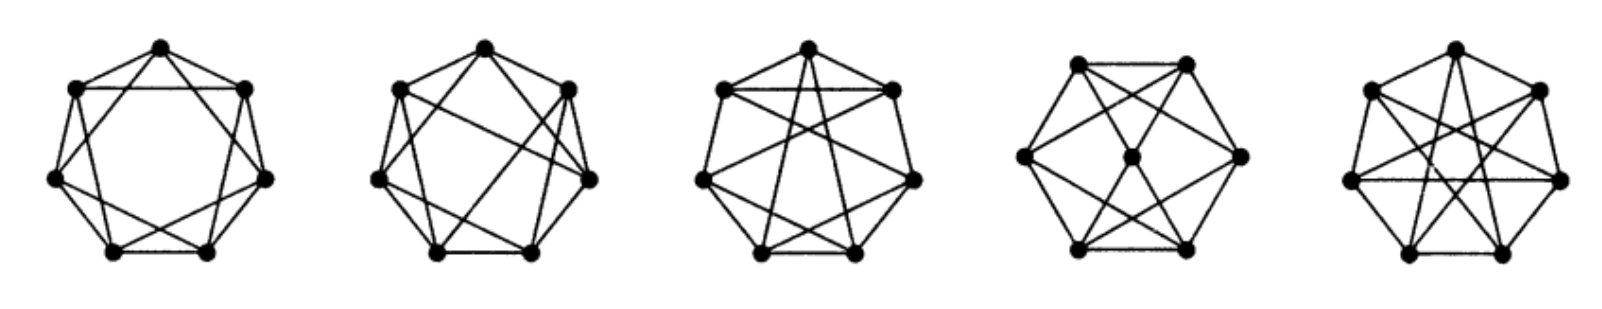
\includegraphics[width=0.9\linewidth]{grafos_10.png}
    \end{center}
\end{ejercicio}
\begin{proof}

\end{proof}

\vspace{0.5cm}

\begin{ejercicio}{11}
    Probar que los grafos de abajo son isomorfos al grafo de Petersen. Hacerlo asociándole a los vértices conjuntos de dos elementos de manera tal que la regla de adyacencia entre vértices sea la misma que en la definición del grafo de Petersen.
    \begin{center}
        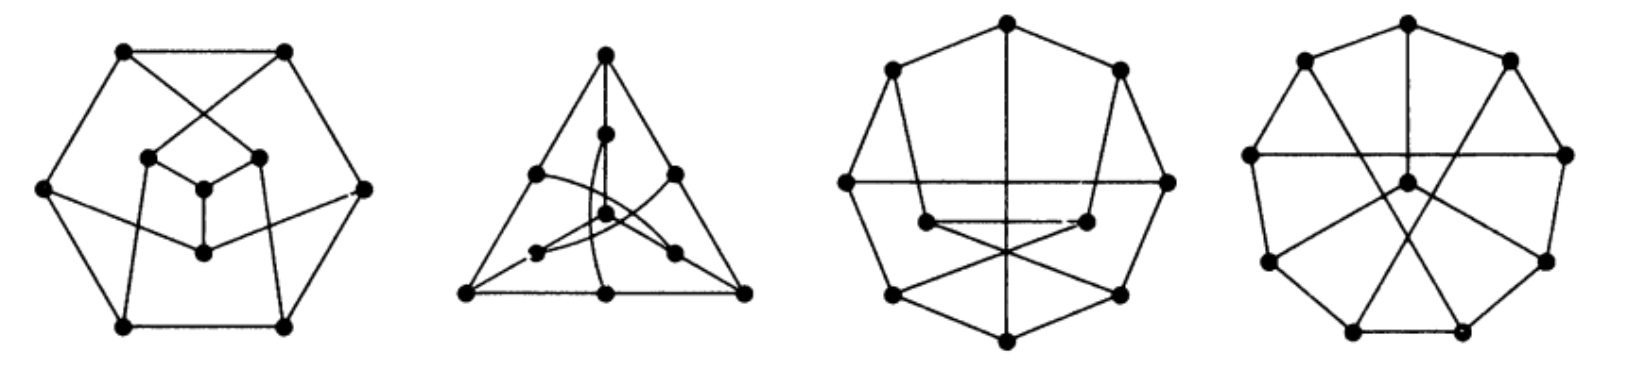
\includegraphics[width=0.9\linewidth]{grafos_11.png}
    \end{center}
\end{ejercicio}
\begin{proof}

\end{proof}

\vspace{0.5cm}

\end{document}